\section{Materiales y métodos}
Los métodos de muestreo, como larvitrampas y ovitrampas resultan eficientes y económicos para
determinar determinar la distribución espacial y temporal de Aedes aegypti y otros mosquitos
\cite{dengueUruguayCap1, cenaprece2013}. La distribución geográfica de larvitrampas, consideradas
como puntos de control, permiten generar información regionalizada sobre el estado de las
poblaciones del vector \cite{NINO2011}, en donde esta información puede ser combinada con
información ambiental, demográfica o epidemiológica, con el fin de obtener modelos detallados que
tengan la capacidad de monitorear, simular el comportamiento del vector y en consecuencia,
predecir una posible epidemia del dengue.

El modelo considera un espacio bi-dimensional, con un sistema de coordenadas geográficas $(x,y)$,
para expresar todas las posiciones sobre el plano, correspondientes a la longitud y latitud. Si
consideramos a $m_{i}$ como a un individuo que se encuentra en una etapa del ciclo de vida del
Aedes aegypti, correspondiente a una población de mosquitos, entonces, $m_{i}(x,y)$ representa a
$m_{i}$ en las coordenadas geográficas $(x,y)$.

Consideramos seis poblaciones diferentes: los huevos $H(x,y)$, larvas $L(x,y)$, pupas $P(x,y)$,
machos adultos $AM(x,y)$, hembras adultas nulíparas\footnote{Hembras que no han ovipuesto.}
$AN(x,y)$ y hembras adultas paridas\footnote{Hembras que han ovipuesto al menos una vez.} $AP(x,y)$. En algunos procesos se utiliza $A(x, y)$ para representar a toda la población de adultos,
$AM(x,y)$, $AN(x,y)$ y $AP(x,y)$ correspondientes a $(x, y)$.

La evolución de las poblaciones, $H(x,y)$, $L(x,y)$, $P(x,y)$, $AM(x,y)$, $AN(x,y)$ y $AP(x,y)$ ,
se ven afectadas por los siguientes eventos: muerte de huevos, eclosión de huevos, muerte de
larvas, emergencia de pupas, muerte de pupas, emergencia de adultos, muerte de adultos, ovipostura
de hembras nulíparas, ovipostura de hembras paridas y dispersión de los adultos (machos y hembras).
Según \cite{otero2006stochastic} los eventos se producen a tasas que dependen no sólo de valores
de la población, sino también de la temperatura, que a su vez es una función de tiempo, por lo
tanto, la dependencia de la temperatura introduce una dependencia del tiempo en las tasas de
eventos. La evolución es modelada como un proceso iterativo diario, en donde la ocurrencia de los
eventos mencionados anteriormente están sujetos a las temperaturas $k_{i}$ reportadas diariamente
en un periodo de tiempo $\vec{k}$.

\subsection{Tasas de desarrollo}
En el modelo se cuenta con 4 tasas de desarrollos correspondientes a : la eclosión de huevos,
emergencia a pupas, emergencia a adultos y el ciclo gonotrófico. Estos valores son obtenidos
mediante el modelo no lineal de Sharpe y DeMichele, presentado en \cite{sharpe1977reaction}, para procesos poiquilotermos\footnote{ La poiquilotermia o ectotermia es un término aplicado a ciertos
animales con temperatura corporal variable}, donde el el proceso de maduración es controlado por
una enzima que actúa en un rango de temperatura determinado, la enzima se desactiva a las bajas temperaturas, $TL$, y altas $TH$.

\begin{equation} \label{eq:schoolfield}
   R(k)  = R(298K) *\cfrac{ \cfrac{k}{298K} *
    exp \Bigg[
            \cfrac{\Delta H_{A}}{R} \bigg(\cfrac{1}{298K} - \cfrac{1}{k}\bigg)
        \Bigg]}
    {1 + exp\Bigg[\cfrac{\Delta H_{H}}{R} \bigg(\cfrac{1}{T_{1/2}}- \cfrac{1}{k}\bigg)\Bigg] }
\end{equation}

Donde $R(k)$ representa la tasa de desarrollo media ($dias^{-1}$) para una temperatura $K$,en la
escala de Kelvin; $T_{H}$ , $T_{L}$ son temperaturas absolutas, en la escala de Kelvin, mientras
que $H_{A}$, $H_{H}$ y $H_{L}$ son entalpías termodinámicas características del organismo, y $R$,
igual $1,987202$ $cal/K.mol$, es la constante universal de los gases.

Donde $T_{1/2}$ es la temperatura cuando la mitad de la enzima se desactiva, debido a la alta
temperatura. Los parámetros $R(298K)$, $H_{A}$, $T_{1/2}$, y $H_{H}$ son estimados mediante la
de regresión no lineal de Wagner, presentado en \cite{wagner1984modeling}. Para este trabajo,
al igual que \cite{rueda1990temperature, otero2006stochastic}, se adopta el modelo de Schoolfield,
ya que, según \cite{otero2006stochastic}, es lo suficientemente flexible para el ajuste de los
datos biológicos disponibles. Los parámetros deben calcularse para cada etapa de desarrollo, una
vez determinados, la ecuación puede utilizarse para calcular tasas de desarrollo a cualquier
temperatura \cite{rueda1990temperature}.

\subsection{Mortalidad}
\label{subsec:cap4-mortalidad}
La mortalidad de los individuos depende de la etapa del ciclo de desarrollo en el que se encuentren
los individuos de una población.


\subsubsection{Mortalidad de huevos}
La tasa de mortalidad de los huevos se encuentra definida como una constante, $me = 0.01$,
$1/\text{días}$, independiente de la temperatura \cite{otero2006stochastic}.

\begin{equation}
    M_{H(x,y)} = \rho(me * H(x,y))
\end{equation}

Donde $M_{H(x,y)}$ es la cantidad de huevos que deben ser eliminados de la población $H(x,y)$.

\subsubsection{Mortalidad de larvas}
La mortalidad de las larvas, según \cite{otero2006stochastic}, se encuentra dividida en dos
contribuciones. La primera contribución representa la mortalidad natural bajo óptimas condiciones
y se encuentra influenciada únicamente de la temperatura \cite{otero2006stochastic}. Esta tasa se
encuentra definida por :

\begin{equation}
\label{eq:mortalidad-natural-larvas}
    ml(k) = 0.01 + 0.9725 * exp\bigg( \frac{-(k - 278)}{2.7035}\bigg)
\end{equation}

La segunda contribución es la mortalidad denso dependiente de las larvas \cite{otero2006stochastic}
. Este mecanismo de regulación puede estar relacionado con procesos concurrentes, como las
limitaciones de los alimentos, las interacciones químicas, presencia de depredadores
especializados en el sitio de reproducción y mucho más \cite{otero2006stochastic}. Esta se
encuentra definida por :

\begin{equation}
  \alpha (x,y) = \alpha _{0}/BS(x,y)
\end{equation}

Donde $\alpha _{0}$ está asociado a la capacidad de carga de un solo lugar de reproducción y
$BS(x,y)$ es el número de sitios de reproducción en $(x,y)$. El valor de $\alpha _{0}$ puede ser
instalado en los valores observados en la región que se está simulando.

Tomando ambas contribuciones, la mortalidad natural bajo óptimas condiciones y la denso
dependiente, la mortalidad de las larvas queda definida como :
\begin{equation}
    M_{L(x,y)}(k) = \rho(ml(k) * L(x,y) + \alpha (x,y) * L(x,y) *(L(x,y) - 1))
\end{equation}

Donde $M_{L(x,y)}$ es la cantidad de larvas que deben ser eliminadas de la población $L(x,y)$.

\subsubsection{Mortalidad de las pupas}
La tasa de mortalidad de las pupas se encuentra definida como una función influenciada únicamente
de la temperatura \cite{otero2006stochastic}.

\begin{equation}
\label{eq:mortalidad-natural-pupas}
    mp(k) = 0.01 + 0.9725 * exp\bigg( \frac{-(k - 278)}{2.7035}\bigg)
\end{equation}

Además de la mortalidad diaria en la fase de pupa, existe una importante mortalidad adicional
asociada con la emergencia sin éxito de adultos, solo el 83\%  de las pupas alcanzan la maduración
y emergerán como mosquitos adultos, por lo tanto, el factor de supervivencia es de $ef=0.83$
\cite{otero2006stochastic}.

\begin{equation}
    M_{P(x,y)}(k) = \rho(P(x,y) * (mp + (1 - ef) * R(k)))
\end{equation}

Donde $M_{P(x,y)}$ es la cantidad de pupas que deben ser eliminadas de la población $P(x,y)$.

\subsubsection{Mortalidad de adultos}
La tasa de mortalidad de los adultos se encuentra definida como una constante, $ma = 0.09$,
$1/\text{días}$, independiente de la temperatura \cite{otero2006stochastic}.

\begin{equation}
    M_{A(x,y)} = \rho(ma * A(x,y))
\end{equation}

Donde $M_{A(x,y)}$ es la cantidad de adultos que deben ser eliminados de la población $A(x,y)$.

\subsection{Ciclo gonotrófico y Ovipostura}
El ciclo gonotrófico de los mosquitos es el nombre que se le adjudicó al período que existe desde
que el mosquito realiza una alimentación sanguínea - ovipostura - hasta una nueva alimentación.
Como se mencionó anteriormente, la tasa de desarrollo del ciclo gonotrófico puede estimarse mediante la versión simplificada del modelo de Sharpe y DeMichele \cite{sharpe1977reaction}, propuesta por Schoolfield en \cite{schoolfield1981non}.

Sea $R(k_{i})$ la tasa de desarrollo (ver ecuación \eqref{eq:schoolfield}) del ciclo gonotrófico
de una hembra (nulípara o parida), para una temperatura de $k_{i}$ Kelvin en un instante $i$, se
considera que un día es de ovipostura si se cumple :
\begin{equation}
\label{eq:ciclo-gonotrofico-ovipostura}
    \sum_{i=0}^{N} R(k_{i}) \geq 1
\end{equation}

Donde $N$ es la duración en días del ciclo gonotrófico de la hembra adulta. Para $R(k)$ se aplican
los parámetros correspondientes a hembras nulíparas y paridas de acuerdo al estado de la hembra.
En \cite{edman1987host} se observó que hembras nulíparas de Aedes aegypti poseen un proceso de
digestión más lento en las hembras paridas y por ende el ciclo gonotrófico de las mismas tiende
a ser más largo. La cantidad de huevos en cada oviposición, luego de las alimentaciones sanguíneas
correspondientes, varía entre 30 y 100 unidades \cite{luevano1993ciclo, beltran2001bionomia,cabezas2005dengue}.


\subsection{Zonificación}
\label{subsec:cap4-zonificacion}
Cada entorno puede contar con factores que lo hagan más o menos apto para el desarrollo,
mortalidad, alimentación, dispersión, y reproducción de individuos. En esta sección, con el fin de
simplificar ciertos aspectos muy específicos que se encuentran fuera del alcance de este trabajo,
realizaremos ciertas hipótesis generales, justificadas para este caso de aplicación, pero puede
requerir una revisión en caso general. Estas hipótesis son, los valores observados en un
conjunto de puntos de control, pertenecientes a una zona, permiten la caracterización de dicha
zona como más o menos apta para desarrollo, mortalidad, alimentación, dispersión, y reproducción de
individuos. También consideramos que el tamaño de la zona, y por ende la cantidad de puntos de
control que pertenecen a ella, influye en la caracterización de las zonas.

La zonificación surge ante necesidad de dividir el espacio de estudio de una forma más granular,
para identificar a los individuos que pertenecen a zonas aptas y los que no. Los puntos de control
distribuidos en un área de estudio permiten estimar los niveles de riesgo e infestación
correspondiente a la abundancia de larvas por litro observadas.

Para determinar el tipo de zona de un individuo $m_{i}$ ubicado en $(x,y)$, primero se estima la
densidad relativa de larvas, para $m_{i}(x,y)$, utilizando interpolación espacial y posteriormente
se la clasifica utilizando una escala. Si consideramos a $u(x,y)$ el valor interpolado para
$m_{i}(x,y)$, entonces la densidad relativa de larvas de $m_{i}(x,y)$ es igual a $u(x,y)$. La
cantidad de larvas observadas en los puntos de control, pertenecientes a la zona de $m_{i}(x,y)$,
corresponden a los valores conocidos utilizados para la interpolación espacial, donde el tamaño de
la zona de $m(x,y)$ se encuentra determinado por $r$, que representa el radio una circunferencia
que tiene como centro a $(x,y)$. El tamaño de $r$, es un parámetro ajustable del modelo, mientras
más grande sea el tamaño de $r$, más puntos de control serán considerados para el cálculo de
$u(x,y)$.

El valor estimado de $u(x,y)$ es utilizado para clasificar la zona como \textit{Pésima},
\textit{Mala}, \textit{Regular}, \textit{Buena} u \textit{Óptima} con influencia positiva el
desarrollo, alimentación, dispersión, y reproducción de individuos y negativamente para la
mortalidad. Con la finalidad de utilizar un mismo criterio de clasificación para todos los
individuos, se define una escala única para este caso de estudio. Los valores de dicha escala son
agrupados por la capacidad de generar hembras adultas que eventualmente puedan llegar a oviponer.

Considerando que $u(x,y)$ representa densidad de relativa de larvas y que la escala a utilizar
para su clasificación se basa en su etapa adulta, se debe realizar una transición de los estados
larva a pupa y de pupa a adulto. Esta transición entre estados es necesaria para poder estimar la
cantidad de hembras adultas con capacidad reproductiva. Para realizar los cálculos
correspondientes hay que tener en cuenta las siguientes consideraciones :

\begin{itemize}
    \item Solo el $50$ \% de las larvas observadas son hembras \cite{otero2006stochastic, manrique1998desarrollo}.
    \item La temperatura media anual es de 25 \textcelsius \cite{website:mspbsHistoria2014}.
    \item La tasa mortalidad diaria natural de las larvas y pupas bajo optimas condiciones, a 25 \textcelsius, es igual a $0,01056$ 1/días, según las ecuaciones \eqref{eq:mortalidad-natural-larvas} y \eqref{eq:mortalidad-natural-pupas} respectivamente.
    \item La tasa de desarrollo, a 25 \textcelsius, de la larva hasta su emergencia a adulto es de $11,57$ días \cite{rueda1990temperature}.
    \item El $32,10$ \% de las hembras adultas no oviponen \cite{osoriopontificia}.
\end{itemize}

Estas consideraciones ayudan a simplificar la simulación de la transición de estados pasando de
larva a pupa y de pupa a adulto, con el fin de construir la escala de clasificación. Los valores
de cantidad de hembras con capacidad de oviponer, finalmente obtenidas a partir de $u(x,y)$ son
calculados para un entorno óptimo.



\subsection{Vuelo y dispersión}
El Aedes aegypti es un mosquito doméstico que generalmente esta confinado a las casas donde se
cría \cite{luevano1993ciclo}, tiende a permanecer físicamente en donde emergió, siempre y cuando
no exista algún factor que la perturbe o no disponga de huéspedes, sitios de reposo y de postura
\cite{ThironIzcazaJ2003}. Por lo general, el mosquito, no sobrepasa los 50 a 100 metros durante su
vida \cite{cabezas2005dengue}. En caso de no contar con sitios adecuados de ovipostura y
disponibilidad de alimento tienden a dispersarme una mayor distancia, hasta tres kilómetros, en
busca de mejores condiciones \cite{ThironIzcazaJ2003}. Los mosquitos tienen la particularidad de
volar en sentido contrario a la dirección al viento \cite{ThironIzcazaJ2003,web-site:speedAnimals}
y a una velocidad máxima de 2 kilómetros por hora \cite{web-site:speedAnimals,kaufmann2004flight}.

Partiendo de las hipótesis realizadas en la podemos considerar
que la dispersión se encuentra influenciada por el valor de $u(x,y)$, de ese modo a medida que
$u(x,y)$ varíe, la dispersión debe ajustarse a su tipo de zona. De forma simplificada definimos que
la dispersión de un adulto que se encuentre en zonas del tipo \textit{Regular}, \textit{Buena} u
\textit{Óptima} se encuentra entre 0 y 100 metros de vuelo. Para las hembras adultas, que
pertenezcan a zonas del tipo \textit{Mala} o \textit{Pésima} se tiene una dispersión entre 100 a
3.000 metros de vuelo, de este modo, las hembras adultas que se encuentren en zonas menos aptas
tenderán a desplazarse en busca de mejores condiciones.


\subsection{Simulación del proceso evolutivo}
La simulación del proceso evolutivo del mosquito del Aedes aegypti, presentado previamente en la
, es el encargado de simular los efectos temperatura
en el ciclo de vida del mosquito.

La población inicial es obtenida mediante la cantidad de larvas observadas en los puntos de
control que corresponden a la muestra utilizada para el estudio. Por cada larva observada,
en un punto de control ubicado en las coordenadas geográficas, $(x, y)$, se inicializa un individuo
con las mismas coordenadas del punto de control de origen.

\begin{figure}[!t]
\centering
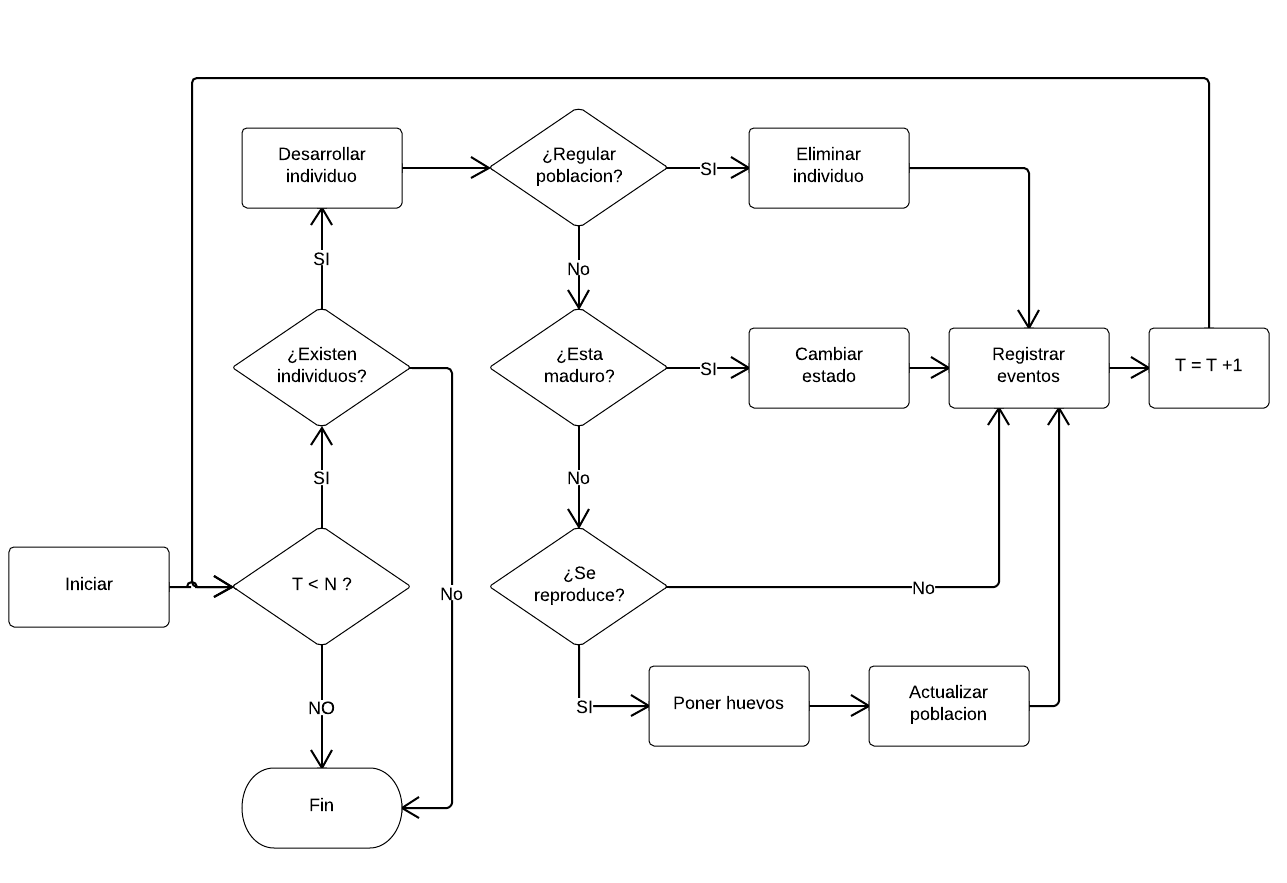
\includegraphics[width=0.45\textwidth]{graphics/algoritmo-evolutivo.png}
\caption{\label{fig:cap-5-alg-evolutivo} Algoritmo del simulador del proceso evolutivo.}
\end{figure}

En la \figref{fig:cap-5-alg-evolutivo}, se presenta el algoritmo del simulador del proceso
evolutivo, que es considerado como un proceso iterativo. El simulador inicia tomando como
parámetros de entrada la población inicial, y el periodo de simulación, representado por $T$. El
proceso se ejecutará siempre y cuando se cumplan las siguientes condiciones : el periodo de
simulación, $T$, no haya finalizado y que la población cuente con individuos para su procesamiento.
En el caso de que no se cumplan algunas de las condiciones mencionadas anteriormente, el proceso
de simulación finalizará.

El desarrollo de los individuos se encarga de calcular las tasas de desarrollo correspondientes
para cada etapa de su ciclo de vida , con el fin de estimar su desarrollo considerando las condiciones climáticas. El cambio de
estado es consecuencia de la finalización de la etapa de desarrollo del individuo, donde el
individuo ya está listo para pasar a la siguiente etapa de su ciclo de desarrollo.


La regulación de la población es la encargada de calcular las tasas de mortalidad diaria,
correspondientes a cada etapa del ciclo de desarrollo del individuo
, con el fin de reducir el tamaño de la población debido a la
mortalidad diaria de los individuos.

Si el individuo en cuestión corresponde a una hembra adulta inseminada, entonces esta se encuentra
en fase reproductiva. La postura de huevos se realiza respetando la tasa de desarrollo del ciclo
gonotrófico de las hembras . Si la hembra
adulta ovipone, los huevos son añadidos a la población como individuos en un estado inicial de
\textit{HUEVO}.

Las efectos de la temperatura, en cada individuo son registrados mediante un proceso que se
encarga de almacenar, en una base de datos, la información correspondiente, de cada individuo para
su posterior análisis. Estos efectos pueden desencadenar en una serie de eventos en el individuo
como : eclosión de huevos, mortalidad de larvas, emergencia de pupas, muerte de pupas, emergencia
de adultos, muerte de adultos, ovipostura y dispersión de los adultos.s
